\chapter{Implementación}
\label{cap:implementacion}

Este capítulo reúne la implementación de todos los componentes del trabajo, el registro LFSR, el algoritmo de Berlekamp-Massey,
los cuatro generadores y los ocho tests del estándar NIST SP 800-22. Para cada uno se muestra el código real
y un ejemplo de ejecución que comprueba que funciona como se espera. La explicación conceptual de cada componente
está en los capítulos anteriores, aquí el foco es el código.

\section{El registro LFSR}

La clase \texttt{LFSR} mantiene el estado como una lista de bits y expone los métodos imprescindibles, \texttt{next\_bit} para avanzar un ciclo,
\texttt{generate} para producir varios bits y \texttt{full\_cycle} para extraer un periodo completo.

\begin{lstlisting}[style=Python,caption={Núcleo de la clase LFSR (\texttt{src/lfsr.py}).}]
class LFSR:
    def __init__(self, taps: list[int], initial_state: list[int]):
        self.degree = max(taps)
        self.taps = taps
        self.state = list(initial_state)
        self._initial_state = list(initial_state)

    def _feedback_bit(self) -> int:
        result = 0
        for t in self.taps:
            result ^= self.state[t - 1]
        return result

    def next_bit(self) -> int:
        output = self.state[-1]
        new_bit = self._feedback_bit()
        self.state = [new_bit] + self.state[:-1]
        return output

    def generate(self, n: int) -> list[int]:
        return [self.next_bit() for _ in range(n)]

    def full_cycle(self) -> list[int]:
        sequence = []
        while True:
            sequence.append(self.next_bit())
            if self.state == self._initial_state:
                break
        return sequence
\end{lstlisting}

Para comprobar que funciona, ejecutamos el script con el mismo LFSR del ejemplo del capítulo~\ref{cap:fundamentos},
grado 3 y polinomio $x^3 + x + 1$ con estado inicial $[1, 0, 0]$.
Esperamos un periodo de $2^3 - 1 = 7$ y la secuencia $\{0, 0, 1, 1, 1, 0, 1\}$ que sacamos a mano.

\begin{figure}[H]
\centering
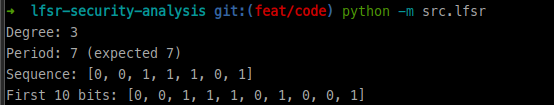
\includegraphics[width=0.9\textwidth]{images/execution_lfsr.png}
\caption{Salida de \texttt{python -m src.lfsr}.}
\label{fig:exec-lfsr}
\end{figure}

El periodo coincide con el teórico y la secuencia es exactamente la que calculamos a mano.
Esta es la base sobre la que se construyen los generadores.

\section{Berlekamp-Massey}

La implementación de Berlekamp-Massey recorre la secuencia bit a bit, mantiene un LFSR candidato y lo ajusta
cuando aparece una discrepancia, devolviendo el grado del LFSR mínimo y su polinomio de conexión.

\begin{lstlisting}[style=Python,caption={Implementación de Berlekamp-Massey (\texttt{src/berlekamp\_massey.py}).}]
def berlekamp_massey(sequence: list[int]) -> tuple[int, list[int]]:
    """Returns (linear_complexity, connection_polynomial)."""
    n = len(sequence)
    s = sequence[:]

    C = [1]
    B = [1]
    L = 0
    m = 1

    for i in range(n):
        d = s[i]
        for j in range(1, L + 1):
            if j < len(C):
                d ^= C[j] & s[i - j]
        d &= 1

        if d == 0:
            m += 1
        elif 2 * L <= i:
            T = C[:]
            padding = [0] * m
            shifted_B = padding + B
            while len(C) < len(shifted_B):
                C.append(0)
            for j in range(len(shifted_B)):
                C[j] ^= shifted_B[j]
            L = i + 1 - L
            B = T
            m = 1
        else:
            padding = [0] * m
            shifted_B = padding + B
            while len(C) < len(shifted_B):
                C.append(0)
            for j in range(len(shifted_B)):
                C[j] ^= shifted_B[j]
            m += 1

    return L, C
\end{lstlisting}

En la práctica. Generamos 20 bits con un LFSR de grado 5 (polinomio $x^5 + x^2 + 1$) y se lo pasamos a Berlekamp-Massey,
incluyendo una segunda llamada con solo los 10 primeros bits.

\begin{figure}[H]
\centering
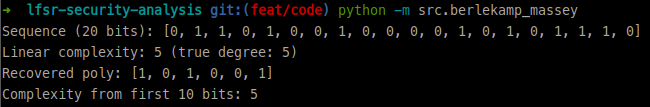
\includegraphics[width=0.9\textwidth]{images/execution_bm.png}
\caption{Salida de \texttt{python -m src.berlekamp\_massey}.}
\label{fig:exec-bm}
\end{figure}

El algoritmo recupera el grado real (5) y el polinomio correcto. Y con solo 10 bits ya converge, porque $2 \cdot 5 = 10$,
justo lo que predice la teoría.

\section{Generador de Geffe}

\begin{lstlisting}[style=Python,caption={Generador de Geffe (\texttt{src/generators/geffe.py}).}]
def geffe_generator(r1: LFSR, r2: LFSR, r3: LFSR, n: int) -> list[int]:
    """Generates n bits using the Geffe generator."""
    output = []
    for _ in range(n):
        a = r1.next_bit()
        b = r2.next_bit()
        c = r3.next_bit()
        output.append((a & b) ^ ((1 ^ a) & c))
    return output
\end{lstlisting}

La función booleana equivalente es $(a \wedge b) \oplus (\neg a \wedge c)$, que es la forma estándar de un multiplexor.

Ejecutamos el generador con los polinomios $R_1$ de grado 7, $R_2$ de grado 5 y $R_3$ de grado 9 (todos primitivos),
sobre una secuencia de 1000 bits, midiendo la complejidad lineal con Berlekamp-Massey.

\begin{figure}[H]
\centering
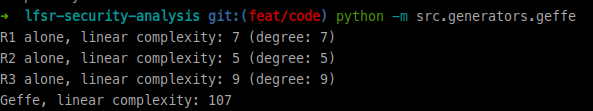
\includegraphics[width=0.9\textwidth]{images/execution_geffe.png}
\caption{Salida de \texttt{python -m src.generators.geffe}.}
\label{fig:exec-geffe}
\end{figure}

La complejidad lineal pasa de los grados originales (7, 5, 9) a 107. Hay una mejora clara, pero como se explica
en el capítulo~\ref{cap:generadores}, la complejidad lineal alta no salva al generador.

\section{Generador Shrinking}

\begin{lstlisting}[style=Python,caption={Generador Shrinking (\texttt{src/generators/shrinking.py}).}]
def shrinking_generator(r1: LFSR, r2: LFSR, n: int) -> list[int]:
    """Generates n bits. r1 filters the output of r2."""
    output = []
    max_clocks = n * 10
    clocked = 0

    while len(output) < n and clocked < max_clocks:
        a = r1.next_bit()
        b = r2.next_bit()
        clocked += 1
        if a == 1:
            output.append(b)

    if len(output) < n:
        raise RuntimeError(
            f"could not generate {n} bits after {max_clocks} clocks"
        )

    return output
\end{lstlisting}

El parámetro \texttt{max\_clocks} es una protección, si por algún motivo $R_1$ produjera demasiados ceros consecutivos,
el bucle terminaría con un error en vez de quedarse colgado.

Ejecutamos el generador con los mismos parámetros que antes,
$R_1$ grado 7 y $R_2$ grado 5, generando 1000 bits.

\begin{figure}[H]
\centering
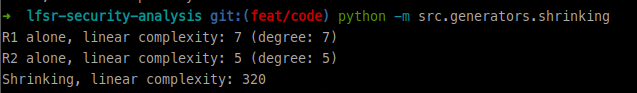
\includegraphics[width=0.9\textwidth]{images/execution_shrinking.png}
\caption{Salida de \texttt{python -m src.generators.shrinking}.}
\label{fig:exec-shrinking}
\end{figure}

El salto es enorme. De LFSR de grados 7 y 5 (que individualmente tendrían complejidad lineal 7 y 5),
salimos con una complejidad lineal de 320. El factor de mejora frente al LFSR más grande es de unos 45x.
Y a diferencia de Geffe, no hay correlación directa explotable, ya que un atacante no sabe en qué posición del ciclo de $R_2$ está cada bit de la salida.

\section{Generador Self-Shrinking}

\begin{lstlisting}[style=Python,caption={Generador Self-Shrinking (\texttt{src/generators/self\_shrinking.py}).}]
def self_shrinking_generator(r: LFSR, n: int) -> list[int]:
    """Generates n bits from a single LFSR using self-shrinking."""
    output = []
    max_clocks = n * 10
    clocked = 0

    while len(output) < n and clocked < max_clocks:
        a = r.next_bit()
        b = r.next_bit()
        clocked += 2
        if a == 1:
            output.append(b)

    if len(output) < n:
        raise RuntimeError(
            f"could not generate {n} bits after {max_clocks} clocks"
        )

    return output
\end{lstlisting}

Ejecutamos sobre un LFSR de grado 11 con polinomio $x^{11} + x^2 + 1$, generando 1000 bits.

\begin{figure}[H]
\centering
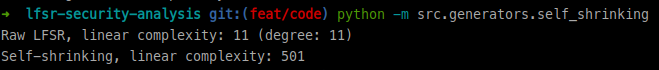
\includegraphics[width=0.9\textwidth]{images/execution_self_shrinking.png}
\caption{Salida de \texttt{python -m src.generators.self\_shrinking}.}
\label{fig:exec-self-shrinking}
\end{figure}

De nuevo el salto es enorme, de 11 a 501, factor 45x. La complejidad lineal queda en valores similares al Shrinking con menos hardware.

\section{Alternating Step Generator (ASG)}

\begin{lstlisting}[style=Python,caption={Generador ASG (\texttt{src/generators/alternating\_step.py}).}]
def alternating_step_generator(r1: LFSR, r2: LFSR, r3: LFSR, n: int) -> list[int]:
    """Generates n bits. r1 decides which of r2/r3 advances."""
    output = []

    b2 = r2.next_bit()
    b3 = r3.next_bit()

    for _ in range(n):
        a = r1.next_bit()
        if a == 1:
            b2 = r2.next_bit()
        else:
            b3 = r3.next_bit()
        output.append(b2 ^ b3)

    return output
\end{lstlisting}

Una sutileza, los bits $b_2$ y $b_3$ se inicializan fuera del bucle. Esto es necesario porque en cada iteración solo se avanza uno de los dos,
así que el otro tiene que tener un valor previo válido para entrar en el XOR.

Ejecutamos el generador con los mismos LFSR que usamos en Geffe,
grados 7, 5 y 9 con 1000 bits de salida.

\begin{figure}[H]
\centering
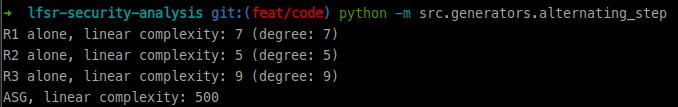
\includegraphics[width=0.9\textwidth]{images/execution_alternating_step.png}
\caption{Salida de \texttt{python -m src.generators.alternating\_step}.}
\label{fig:exec-asg}
\end{figure}

Esto es lo más interesante de todo el capítulo. Con los mismos LFSR que dieron 107 de complejidad lineal en Geffe,
el ASG llega a 500. La diferencia no está en los registros ni en sus tamaños sino exclusivamente
en cómo se combinan sus salidas. Reloj alterno y XOR de fuentes independientes amplifica mucho más la complejidad lineal que un multiplexor.

\section{Tests aplicados}

De los quince tests del estándar NIST SP 800-22 se implementan ocho.
Los siete restantes (cumulative sums, random excursions y variantes, approximate entropy,
overlapping template matching y longest run of ones) requieren secuencias considerablemente más largas
o evalúan propiedades que en el contexto de LFSR son redundantes con las que ya cubrimos.

\subsection{Test de frecuencia (Monobit)}

Comprueba si la proporción de unos y ceros en la secuencia se acerca al 50\%.
El estadístico convierte los bits a $\pm 1$, los suma y mira si el resultado está cerca de cero.

\begin{lstlisting}[style=Python,caption={Test Monobit (\texttt{src/tests\_nist/monobit.py}).}]
def monobit_test(sequence: list[int]) -> tuple[float, bool]:
    n = len(sequence)
    if n < 100:
        raise ValueError("sequence too short, need at least 100 bits")

    S_n = sum(1 if b == 1 else -1 for b in sequence)
    s_obs = abs(S_n) / math.sqrt(n)
    p_value = math.erfc(s_obs / math.sqrt(2))

    return p_value, p_value >= 0.01
\end{lstlisting}

Es el test más básico, si una secuencia tiene un sesgo claro hacia uno de los dos valores,
este test lo detecta. Pasarlo es condición necesaria pero está lejos de ser suficiente.

\subsection{Test de frecuencia en bloques}

Versión más detallada del monobit. Divide la secuencia en bloques de longitud $M$ y comprueba si la proporción de unos dentro de cada bloque se acerca a $1/2$.
Detecta desequilibrios locales que el monobit global no vería.

\begin{lstlisting}[style=Python,caption={Test Block Frequency (\texttt{src/tests\_nist/block\_frequency.py}).}]
def block_frequency_test(sequence: list[int], block_size: int = 128) -> tuple[float, bool]:
    n = len(sequence)
    num_blocks = n // block_size

    proportions = []
    for i in range(num_blocks):
        block = sequence[i * block_size : (i + 1) * block_size]
        pi_i = sum(block) / block_size
        proportions.append(pi_i)

    chi_sq = 4 * block_size * sum((pi - 0.5) ** 2 for pi in proportions)
    p_value = _igamc(num_blocks / 2, chi_sq / 2)

    return p_value, p_value >= 0.01
\end{lstlisting}

En los experimentos uso bloques de 128 bits, que es el valor recomendado por defecto del estándar.

\subsection{Test de rachas}

Una racha es una subsecuencia maximal de bits consecutivos iguales,
por ejemplo en $\{1, 1, 0, 0, 0, 1\}$ hay tres rachas.
El test comprueba si el número total de rachas es coherente con una secuencia aleatoria.
Demasiadas rachas indican oscilación excesiva, pocas indican bloques largos de bits iguales.

\begin{lstlisting}[style=Python,caption={Test de rachas (\texttt{src/tests\_nist/runs.py}).}]
def runs_test(sequence: list[int]) -> tuple[float, bool]:
    n = len(sequence)
    pi = sum(sequence) / n

    tau = 2 / math.sqrt(n)
    if abs(pi - 0.5) >= tau:
        return 0.0, False

    V_n = 1 + sum(
        1 for k in range(n - 1) if sequence[k] != sequence[k + 1]
    )

    numerator = abs(V_n - 2 * n * pi * (1 - pi))
    denominator = 2 * math.sqrt(2 * n) * pi * (1 - pi)
    p_value = math.erfc(numerator / denominator)

    return p_value, p_value >= 0.01
\end{lstlisting}

El test tiene un prerrequisito de balance, si la proporción de unos está muy lejos de $0{,}5$,
no tiene sentido calcular el estadístico y se devuelve p-valor 0 directamente.

\subsection{Test de rango de matriz binaria}

Toma chunks consecutivos de la secuencia, los reorganiza en matrices $32 \times 32$ y calcula su rango con XOR.
En una secuencia aleatoria, las matrices tienden a tener rango completo con una probabilidad conocida.
En secuencias con estructura lineal el rango es menor.

\begin{lstlisting}[style=Python,caption={Test Binary Matrix Rank (extracto de \texttt{src/tests\_nist/binary\_matrix.py}).}]
def binary_matrix_rank_test(sequence: list[int], rows: int = 32, cols: int = 32):
    n = len(sequence)
    block_size = rows * cols
    num_matrices = n // block_size

    F_M = 0; F_M1 = 0; F_rem = 0
    for i in range(num_matrices):
        block = sequence[i * block_size : (i + 1) * block_size]
        matrix = [block[r * cols : (r + 1) * cols] for r in range(rows)]
        rank = _gf2_rank(matrix)

        if rank == rows:
            F_M += 1
        elif rank == rows - 1:
            F_M1 += 1
        else:
            F_rem += 1

    chi_sq = (
        (F_M - num_matrices * 0.2888) ** 2 / (num_matrices * 0.2888) +
        (F_M1 - num_matrices * 0.5776) ** 2 / (num_matrices * 0.5776) +
        (F_rem - num_matrices * 0.1336) ** 2 / (num_matrices * 0.1336)
    )
    p_value = math.exp(-chi_sq / 2)
    return p_value, p_value >= 0.01
\end{lstlisting}

Este test es especialmente relevante para LFSR, ya que un LFSR de grado $n$ con $n < 32$ tiende a producir matrices con dependencias lineales entre filas
(las filas viven en un subespacio de dimensión a lo sumo $n$), lo que reduce el rango y dispara el chi-cuadrado.

\subsection{Test universal de Maurer}

Mide la compresibilidad de la secuencia. La idea intuitiva es que una secuencia verdaderamente aleatoria no se puede comprimir significativamente porque no hay patrones que aprovechar.
Si la secuencia tiene regularidades (periodicidad, correlaciones a larga distancia), los patrones se repiten con más frecuencia de la esperada.

\begin{lstlisting}[style=Python,caption={Test universal de Maurer (extracto, \texttt{src/tests\_nist/maurer.py}).}]
def maurer_test(sequence: list[int], block_size: int = 6) -> tuple[float, bool]:
    L = block_size
    Q = 10 * (2 ** L)
    n = len(sequence)
    K = n // L - Q

    T = [0] * (2 ** L)
    for i in range(Q):
        block = sequence[i * L : (i + 1) * L]
        idx = int("".join(str(b) for b in block), 2)
        T[idx] = i + 1

    sum_log = 0.0
    for i in range(Q, Q + K):
        block = sequence[i * L : (i + 1) * L]
        idx = int("".join(str(b) for b in block), 2)
        distance = (i + 1) - T[idx]
        sum_log += math.log2(distance)
        T[idx] = i + 1

    f_n = sum_log / K
    expected, variance = _MAURER_TABLE[L]
    c = 0.7 - 0.8 / L + (4 + 32 / L) * (K ** (-3.0 / L)) / 15
    sigma = c * math.sqrt(variance / K)

    p_value = math.erfc(abs(f_n - expected) / (math.sqrt(2) * sigma))
    return p_value, p_value >= 0.01
\end{lstlisting}

En los experimentos uso $L = 6$ que es el valor mínimo recomendado para secuencias del orden de medio millón de bits.

\subsection{Test serial}

Comprueba que todos los patrones de $m$ bits aparezcan con frecuencia similar. Para $m = 3$, los ocho patrones posibles ($000$, $001$, $\ldots$, $111$) deberían aparecer
aproximadamente con la misma frecuencia $1/8$ cada uno.

\begin{lstlisting}[style=Python,caption={Test serial (\texttt{src/tests\_nist/serial.py}).}]
def serial_test(sequence: list[int], block_size: int = 3):
    n = len(sequence)
    m = block_size

    psi_sq_m  = _psi_sq(sequence, n, m)
    psi_sq_m1 = _psi_sq(sequence, n, m - 1)
    psi_sq_m2 = _psi_sq(sequence, n, m - 2) if m >= 2 else 0.0

    del1 = psi_sq_m - psi_sq_m1
    del2 = psi_sq_m - 2 * psi_sq_m1 + psi_sq_m2

    p1 = float(gammaincc(2 ** (m - 2), del1 / 2))
    p2 = float(gammaincc(2 ** (m - 3), del2 / 2)) if m >= 2 else 1.0

    passed = p1 >= 0.01 and p2 >= 0.01
    return (p1, p2), passed
\end{lstlisting}

El test devuelve dos p-valores y los dos tienen que pasar. Para reportar un único valor en las tablas uso el mínimo de los dos.

\subsection{Test espectral (DFT)}

Aplica la transformada discreta de Fourier a la secuencia (convirtiendo previamente los bits a $\pm 1$) y mira si hay picos
anormalmente altos en el espectro de frecuencias, lo que indicaría periodicidades ocultas.

\begin{lstlisting}[style=Python,caption={Test espectral (\texttt{src/tests\_nist/spectral.py}).}]
def spectral_test(sequence: list[int]) -> tuple[float, bool]:
    n = len(sequence)
    x = np.array([1 if b == 1 else -1 for b in sequence], dtype=float)

    X = np.fft.fft(x)
    magnitudes = np.abs(X[: n // 2])

    threshold = math.sqrt(math.log(1 / 0.05) * n)
    N_0 = 0.95 * n / 2
    N_1 = np.sum(magnitudes < threshold)

    d = (N_1 - N_0) / math.sqrt(n * 0.95 * 0.05 / 4)
    p_value = math.erfc(abs(d) / math.sqrt(2))

    return p_value, p_value >= 0.01
\end{lstlisting}

Este test es el que más nos interesa en el contexto de LFSR, ya que las m-sequences tienen periodicidad perfecta y los generadores que muestrean LFSR
pueden conservar componentes frecuenciales del registro original. Como se verá en los resultados, es el test que mejor discrimina entre generadores.

\subsection{Test de complejidad lineal}

Divide la secuencia en bloques de longitud $M$, calcula la complejidad lineal de cada bloque con Berlekamp-Massey y compara la distribución de complejidades observadas
con la teórica para bloques aleatorios.

\begin{lstlisting}[style=Python,caption={Test de complejidad lineal (extracto, \texttt{src/tests\_nist/linear\_complexity.py}).}]
def linear_complexity_test(sequence: list[int], block_size: int = 500):
    n = len(sequence)
    M = block_size
    N = n // M

    mu = M / 2 + (9 + (-1) ** (M + 1)) / 36 - (M / 3 + 2 / 9) / (2 ** M)

    T = []
    for i in range(N):
        block = sequence[i * M : (i + 1) * M]
        L = linear_complexity(block)
        T.append((-1) ** M * (L - mu) + 2 / 9)

    nu = [0] * 7
    for t in T:
        if t <= -2.5: nu[0] += 1
        elif t <= -1.5: nu[1] += 1
        elif t <= -0.5: nu[2] += 1
        elif t <= 0.5: nu[3] += 1
        elif t <= 1.5: nu[4] += 1
        elif t <= 2.5: nu[5] += 1
        else: nu[6] += 1

    pi = [0.010417, 0.03125, 0.125, 0.5, 0.25, 0.0625, 0.020833]
    chi_sq = sum((nu[i] - N * pi[i]) ** 2 / (N * pi[i]) for i in range(7))
    p_value = float(gammaincc(3, chi_sq / 2))
    return p_value, p_value >= 0.01
\end{lstlisting}

Uso bloques de 500 bits, valor estándar. Es el test que tira de Berlekamp-Massey de forma directa,
y por eso el que detecta más limpiamente las secuencias con estructura lineal.
